\documentclass[10pt]{article}
\usepackage{graphicx}
\usepackage{float}
\usepackage{amsmath}
\usepackage{amsfonts}
\usepackage[brazilian]{babel}
\usepackage[utf8]{inputenc}
\usepackage[T1]{fontenc}

%macros
\newcommand{\fromeng}[1]{\footnote{do inglês: \textit{#1}}}
\newcommand{\tit}[1]{\textit{#1}}
\newcommand{\tbf}[1]{\textbf{#1}}
\newcommand{\ttt}[1]{\texttt{#1}}

\begin{document}

\title{MC833 - Tarefa 7}
\author{Erik de Godoy Perillo - RA: 135582}
\maketitle

\begin{enumerate}
\item --
	\begin{itemize}
		\item \ttt{int \tbf{setsockopt}(int sockfd, int level, int optname,
			const void *optval, socklen\_t optlen)}
	\end{itemize}

	Procedimento utilizado para configurar opções para o \tit{socket}
	referido por \ttt{sockopt}. O nível de protocolo no qual a opção existe
	deve ser indicado por \ttt{level}. A opção então é especificada por 
	\ttt{optname}; seu valor é colocado em \ttt{optval} e o tamanho do 
	tipo respectivo ao valor passado é especificado em \ttt{optlen}.

\item Implementado.

\item O cliente permite a opção `u' para usar protocolo UDP ou `t' 
	para TCP\@. Na imagem abaixo pode-se verificar o funcionamento 
	do servidor e clientes. À esquerda, está o servidor. 
	Á direita, de cima pra baixo, estão o cliente novo usando UDP,
	o cliente novo usando TCP, o cliente da tarefa 3 usando TCP e o
	netcat usando UDP, respectivamente.

	\begin{figure}[H]
	\centering
	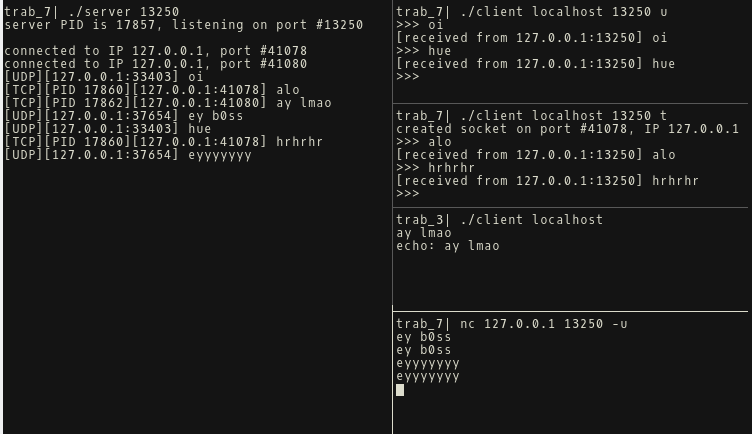
\includegraphics[width=1.0\linewidth]{imgs/q3.png}
	\end{figure}

	Foi comprovada a comunicação via rede através do \tit{tcpdump} Pode-se
	ver que as portas da imagem estão de fato envolvidas, e todos usam o
	protocolo esperado:

	\fbox{\parbox{\textwidth}{
	\ttt{\$ sudo tcpdump -i lo\newline
		08:13:36.795211 IP localhost.localdomain.41078 > localhost.localdomain.13250: Flags [S], seq 919632063, win 43690, options [mss 65495,sackOK,TS val 27266798 ecr 0,nop,wscale 7], length 0\newline
		08:13:36.795223 IP localhost.localdomain.13250 > localhost.localdomain.41078: Flags [S.], seq 3828928855, ack 919632064, win 43690, options [mss 65495,sackOK,TS val 27266798 ecr 27266798,nop,wscale 7], length 0\newline
		08:13:36.795236 IP localhost.localdomain.41078 > localhost.localdomain.13250: Flags [.], ack 1, win 342, options [nop,nop,TS val 27266798 ecr 27266798], length 0\newline
		08:13:37.722931 IP localhost.localdomain.41080 > localhost.localdomain.13250: Flags [S], seq 4212890171, win 43690, options [mss 65495,sackOK,TS val 27267076 ecr 0,nop,wscale 7], length 0\newline
		08:13:37.722942 IP localhost.localdomain.13250 > localhost.localdomain.41080: Flags [S.], seq 2347226256, ack 4212890172, win 43690, options [mss 65495,sackOK,TS val 27267076 ecr 27267076,nop,wscale 7], length 0\newline
		08:13:37.722953 IP localhost.localdomain.41080 > localhost.localdomain.13250: Flags [.], ack 1, win 342, options [nop,nop,TS val 27267076 ecr 27267076], length 0\newline
		08:13:40.552848 IP localhost.localdomain.33403 > localhost.localdomain.13250: UDP, length 4\newline
		08:13:40.552945 IP localhost.localdomain.13250 > localhost.localdomain.33403: UDP, length 4\newline
		08:13:42.052228 IP localhost.localdomain.41078 > localhost.localdomain.13250: Flags [P.], seq 1:6, ack 1, win 342, options [nop,nop,TS val 27268375 ecr 27266798], length 5\newline
		08:13:42.052274 IP localhost.localdomain.13250 > localhost.localdomain.41078: Flags [.], ack 6, win 342, options [nop,nop,TS val 27268375 ecr 27268375], length 0\newline
		08:13:42.052404 IP localhost.localdomain.13250 > localhost.localdomain.41078: Flags [P.], seq 1:6, ack 6, win 342, options [nop,nop,TS val 27268375 ecr 27268375], length 5\newline
		08:13:42.052436 IP localhost.localdomain.41078 > localhost.localdomain.13250: Flags [.], ack 6, win 342, options [nop,nop,TS val 27268375 ecr 27268375], length 0\newline
	}}}

	\fbox{\parbox{\textwidth}{
	\ttt{08:13:45.601653 IP localhost.localdomain.41080 > localhost.localdomain.13250: Flags [P.], seq 1:10, ack 1, win 342, options [nop,nop,TS val 27269440 ecr 27267076], length 9\newline
		08:13:45.601698 IP localhost.localdomain.13250 > localhost.localdomain.41080: Flags [.], ack 10, win 342, options [nop,nop,TS val 27269440 ecr 27269440], length 0\newline
		08:13:45.601833 IP localhost.localdomain.13250 > localhost.localdomain.41080: Flags [P.], seq 1:10, ack 10, win 342, options [nop,nop,TS val 27269440 ecr 27269440], length 9\newline
		08:13:45.601873 IP localhost.localdomain.41080 > localhost.localdomain.13250: Flags [.], ack 10, win 342, options [nop,nop,TS val 27269440 ecr 27269440], length 0\newline
		08:13:45.671417 IP6 localhost.localdomain.37303 > localhost.localdomain.37303: UDP, length 32\newline
		08:13:45.682938 IP6 localhost.localdomain.37303 > localhost.localdomain.37303: UDP, length 24\newline
		08:13:45.685058 IP6 localhost.localdomain.37303 > localhost.localdomain.37303: UDP, length 32\newline
		08:13:45.695834 IP6 localhost.localdomain.37303 > localhost.localdomain.37303: UDP, length 936\newline
		08:13:45.695857 IP6 localhost.localdomain.37303 > localhost.localdomain.37303: UDP, length 376\newline
	}}}


	\fbox{\parbox{\textwidth}{
	\ttt{08:13:45.695866 IP6 localhost.localdomain.37303 > localhost.localdomain.37303: UDP, length 488\newline
		08:13:47.611600 IP localhost.localdomain.unisys-eportal > localhost.localdomain.13250: UDP, length 8\newline
		08:13:47.611647 IP localhost.localdomain.13250 > localhost.localdomain.unisys-eportal: UDP, length 9\newline
		08:13:49.820236 IP localhost.localdomain.33403 > localhost.localdomain.13250: UDP, length 5\newline
		08:13:49.820310 IP localhost.localdomain.13250 > localhost.localdomain.33403: UDP, length 5\newline
		08:13:53.022632 IP localhost.localdomain.41078 > localhost.localdomain.13250: Flags [P.], seq 6:14, ack 6, win 342, options [nop,nop,TS val 27271666 ecr 27268375], length 8\newline
		08:13:53.022677 IP localhost.localdomain.13250 > localhost.localdomain.41078: Flags [P.], seq 6:14, ack 14, win 342, options [nop,nop,TS val 27271666 ecr 27271666], length 8\newline
		08:13:53.022695 IP localhost.localdomain.41078 > localhost.localdomain.13250: Flags [.], ack 14, win 342, options [nop,nop,TS val 27271666 ecr 27271666], length 0\newline
		08:13:57.075914 IP localhost.localdomain.unisys-eportal > localhost.localdomain.13250: UDP, length 9\newline
		08:13:57.075963 IP localhost.localdomain.13250 > localhost.localdomain.unisys-eportal: UDP, length 10\newline
		08:14:05.380738 IP6 localhost.localdomain.37303 > localhost.localdomain.37303: UDP, length 32\newline
		08:14:05.392142 IP6 localhost.localdomain.37303 > localhost.localdomain.37303: UDP, length 24\newline
		08:14:05.393621 IP6 localhost.localdomain.37303 > localhost.localdomain.37303: UDP, length 32\newline
		08:14:05.404212 IP6 localhost.localdomain.37303 > localhost.localdomain.37303: UDP, length 936\newline
		08:14:05.404227 IP6 localhost.localdomain.37303 > localhost.localdomain.37303: UDP, length 376\newline
		08:14:05.404232 IP6 localhost.localdomain.37303 > localhost.localdomain.37303: UDP, length 488\newline
	}}}

\end{enumerate}

\end{document}
